\subsection{Batterie-Antrieb}
%"In der Luftfahrt ist es möglich, direkten Strom zu nutzen. Die direkte Nutzung von
%Elektrizität erfordert Elektromotoren und Stromspeicher an Bord" \cite{dahal2021techno}, wie Batterie oder Brennstoffzellen \cite{dalmia2022powering}.
Eine andere Möglichkeit, Emissionen zu reduzieren, direkten Strom als Antrieb mittels Elektromotoren und Stromspeicher, wie Batterien oder Brennstoffzellen zu nutzen.
Eine einfache Darstellung des Batterie-Antriebs (BA) in der Abbildung \ref{ba} gezeigt.
\begin{figure}[h]
	\centering
	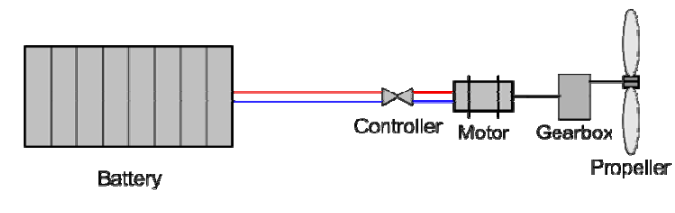
\includegraphics[width=0.7\linewidth]{Bilder/BA.png}
	\caption[Einfachste Batterie-Antrieb]{ \cite{hepperle2012electric}}
	\label{ba}
\end{figure}

Es gibt drei unterschiedliche Antriebskonfigurationen von elektrischen Flugzeugen: vollelektrisch, funktioniert nur auf der Batterie oder
Brennstoffzelle als Energiequelle, turboelektrisch und hybrid-elektrisch ist die Mischung von konventionellen 
Gasturbinentriebwerke mit Kerosin und Batterie oder Brennstoffzelle \cite{dahal2021techno}. %Turboelelektrisches Antrieb 
Im Weiteren wird ein vollelektrisches Antrieb beschrieben.
%
Funktionsweise Elektromotor: Durch Potenzialdifferenz und einen Stromfluss wird die elektrische Energie in die mechanische umgewandelt.
Im Vergleich zum Verbrennungsmotor ist der einzige beweglicher Teil bei BA ist der Rotor \cite{donckers2024electric}, 
was schließlich die Wartungskosten verringern kann. Außerdem besteht der elektrische Antrieb aus Controller, welcher den Energiefluss steuert. 
Durch Controller wird festgelegt, welche Leistung soll der Motor bringen bzw. wie viel Energie soll von 
einer Batterie genommen werden für die gewünschte Leistung \cite{donckers2024electric}. 

Batteriemanagementsystem in einem Flugzeug verfügt über die Information, wie State of Health (SOH), welcher der Unterschied zwischen Anfangs-
und Bestandskapazität eine Batterie anzeigt, und State of Charge (SoC), welcher zeigt, wie viel Prozent der verfügbaren Kapazität geladen werden kann \cite{donckers2024electric}.

%Ein Vorteil des elektrischen Flugzeugs ist, dass den Antrieb zulässt, rückwärtszufahren (Quelle) und somit auf den Schlepper-Einsatz verzichtet werden kann.
Durch die Umwandlung der elektrischen Energie in die chemische kann die Energie in der Batterie gespeichert werden.
Im Laufe des Fluges, die Batterien verändern sein Gewicht nicht, unabhängig davon, ob sie leer oder vollgeladen sind \cite{donckers2024electric}. 
Eine weit verbreitete in der wissenschaftlichen Literatur Batterie ist das Lithium-Ion. Die haben eine hohe Energiedichte im Vergleich zu anderen vorhandenen Batterien. %ist es so?
Heutige Li-ion Batterien haben Energiedichte 100-265 Wh/kg (Quelle). Werden diese Werte zu Kerosins spezifische Energiedichte von 12 kWh/kg verglichen \cite{dalmia2022powering},
das macht Differenz ist ca. 45-mal höher als von einer Li-Ion-Batterie. Das weist darauf hin, dass Batterien viel mehr Gewicht für die gleiche Energie benötigen/haben. Somit steigt auch
die Masse vom Flugzeug.

Die Batterien sind von äußerlichen Bedingungen beeinflussbar. Die kalte Umgebung kann 
der Wirkungsgrad reduzieren (Quelle), und die warme Umgebung kann zu einem schnelleren Auslaufen der Lebensdauer führen.
Die Herstellung der Lithium-Ionen-Batterien ist durch Lithium-Produktion umweltschädlich (was viel Wasser verbraucht, Leckagen gefährlich) und 
kostenintensiv und Wartung \cite{dalmia2022powering}. 

In der Forschung sind weitere Batterien wie Lithium-Sulfur, Lithium-Air, als auch Solid-state Batterien klingen vielversprechend (Quelle).
%
%
%Batterien werden bereits jetzt als sekundäre Leistungsquelle.(Schmidt?)

Batteriewechsel ist kompatibler mit der Flugplanungen, aber benötigt mehreren Batterien für den Austausch, was die Logistik schwerer macht 
und die höheren Anschaffungskosten hat. Batterie sollen richtig und sicher gelagert werden. \cite{salucci2020optimal}

Batteriewechsel ist öfters vorkommende in der Literatur Ladung.

Ladeleistung ist für die Dauer der Ladung verantwortlich. Durch schnellere Ladungen wird Lebensdauer der Batterien reduziert. Was mit sich bringt, dass die Batterien schneller ausgetauscht werden müssen
und mehr Kosten dadurch entsteht. (Quelle) Wobei die langsamen Laden ist für die Fluggesellschaften nicht rentabel sein kann, 
da wenn Flugzeug auf dem Boden steht verdienen Fluggesellschaften kein Geld.

Transportkapazität ist nicht so groß, wie bei konventionellen Flugzeugen und auch die Reichweite für Regionalflüge \cite{abrantes2024impact}.
Die Energieproduktion ist nicht emissionsfrei \cite{abrantes2024impact}, dafür muss mehr erneuerbaren Quellen hergestellt werden, 
wie Solar- und Windenergie. 
%Wasserstoff braucht kryogene Lagerung, hat Entflammbarkeit und braucht Infrastrukturentwicklung.\cite{abrantes2024impact}

In Bezug auf Sicherheit, das größte Gefahr bei BA ist chemische Reaktion des thermischen Durchgehens, wofür stabile
Kühlungssysteme benötigt sind \cite{donckers2024electric}. Thermisches Durchgehen verursacht einen starken Anstieg der 
Innentemperatur von Batterie, was zu kompletten Ausfall der Batterie oder Freisetzung der brennbaren Gase führen kann \cite{shahid2022review}.
%Das thermische Durchgehen von Lithium-Ionen-Batterien ist das Phänomen exothermer Kettenreaktionen innerhalb der Batterie.
% Diese Reaktionen verursachen normalerweise einen starken Anstieg der internen Batterietemperatur, wodurch die inneren Strukturen 
% der Batterie destabilisiert und abgebaut werden, was zu einem Totalausfall der Batterie führen kann. Das thermische Durchgehen kann 
% durch verschiedene Formen mechanischer, elektrischer und thermischer Misshandlung auftreten. All dies führt zu einem internen Kurzschluss 
% der Batterie, da der Separator zwischen Anode und Kathode entweder zusammenbricht, abreißt oder durchbohrt wird. Dadurch wird eine große 
% Menge Wärme erzeugt, die wiederum den Grad der elektrochemischen Reaktionen verstärkt und eine übermäßige Wärmeentwicklung verursacht. 
% Dieser Zyklus setzt sich fort, wodurch die Temperatur der Batterie stark ansteigt und große Mengen brennbarer Gase freigesetzt werden.
